\chapter{K plus proches voisins et apprentissage de métriques}

\myminitoc

\sect{Classification bayésienne}

Le classificateur bayésien prédit la classe optimale $y^*$ d'un exemple $x \in \X$ de la manière suivante :
$$ y^*(x) = \argmax_c \Pp(y_c | x) = \argmax_c \dfrac{\Pp(x | y_c) \Pp(y_c)}{\Pp(x)} = \argmax_c \Pp(x | y_c) \Pp(y_c) $$
Si le calcul de $y^*$ est possible alors le classificateur bayésien est optimal d'un point de vue probabiliste et l'erreur associée est l'erreur de Bayes $\epsilon_B$. \\
Malheureusement, les $\Pp(y_c)$ et les $\Pp(x | y_c)$ sont inconnus. Mais on peut les estimer avec notre ensemble d'entraînement $S$.

\paragraph{\boldmath $\Pp(y_c)$}
Un estimateur non biaisé pour les probabilité des classes est la fréquence d'observation dans l'ensemble $S$ :
$$ \hat{p}(y_c) = \dfrac{|S_c|}{|S|} $$
Où $S_c$ est le nombre d'exemples appartenant à la classe $y_c$ dans l'ensemble $S$.

\paragraph{\boldmath $\Pp(x | y_c)$}
On peut distinguer deux types d'approche.
\begin{itemize}
	\item Les \textbf{méthodes paramétriques} qui assument que $\Pp(x \ y_c)$ suit une certaine loi. Dans ce cas le problème consiste à estimer les paramètres de cette loi. C'est donc une maximisation de la vraisemblance.
	\item Les \textbf{méthodes non paramétriques} qui n'imposent aucune contraintes sur la distribution et pour laquelle les valeurs de $\Pp(x | y_c)$ sont estimés de manière local autour de chaque $x$. La seule supposition sera alors que la distribution est localement régulière.
\end{itemize}

Pour simplifier un peu, on va essayer d'estimer $\Pp(x)$ au lieu de la probabilité $\Pp(x | y_c)$ qui s'obtient simplement en conditionnant l'ensemble d'entraînement $S$ par la classe $y_c$. \\
On considère la probabilité $\mathcal{P}_V$ que $x$ soit dans un volume $V$.
$$ \mathcal{P}_V = \int_V p(x)dx $$
Comme on suppose que $p$ est localement régulier, $p$ varie peu dans le volume $V$ si le volume est suffisamment petit. Pour $x$ dans $V$, on a donc :
$$ \hat{\mathcal{P}}_V \simeq p(x) \times V $$
Mais on peut aussi évaluer $\mathcal{P}$ avec la proportion d'exemples d'entraînement dans $V$. On pose $k_V$ le nombre d'exemple d'entraînement dans $V$ et on a :
$$ \hat{\mathcal{P}}_V \simeq \dfrac{k_V}{m} $$
On en déduit alors, pour $V$ un voisinage de $x$, l'égalité suivante :
$$ \hat{p}(x) = \dfrac{k_V}{m V} $$

\PROP{
	Soit $x \in \X$, et $V_m$ un voisinage de $x$ dans un ensemble de $m$ exemples d'entraînement et $k_m$ la proportion d'exemples de l'ensemble qui sont dans le voisinage $V_m$. \\
	Alors $\hat{p}(x) = \dfrac{k_m}{m V_m}$ converge vers $p(x)$ lorsque $m$ tend vers l'infini si les trois conditions suivantes sont remplies :
	$$ \bullet \lim\limits_{m \rightarrow +\infty} V_m = 0 \qquad \qquad \bullet \lim\limits_{m \rightarrow +\infty} k_m = +\infty \qquad \qquad \bullet \lim\limits_{m \rightarrow +\infty} \dfrac{k_m}{m} = 0$$
	\vspace{-5mm}
}

\paragraph{K plus proches voisins}
Il en vient que les $k$ plus proches voisins satisfont ces propriétés. On fixe un nombre $k_m$ de voisins et on prend un volume $V_m$ qui contient $k_m$ voisins.

\begin{center}
	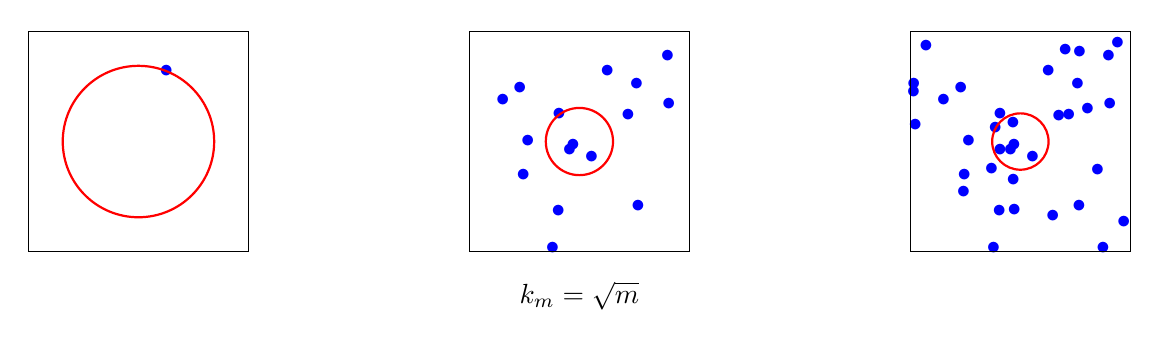
\begin{tikzpicture}[thick, scale=2.8]
		\draw[blue] (0.626252, 0.819381) node {$\bullet$};
		\draw[red] (0.500000, 0.500000) circle (0.343429);
		\draw[blue] (2.626252, 0.819381) node {$\bullet$};
		\draw[blue] (2.766462, 0.208311) node {$\bullet$};
		\draw[blue] (2.265342, 0.502120) node {$\bullet$};
		\draw[blue] (2.555533, 0.427031) node {$\bullet$};
		\draw[blue] (2.403969, 0.184887) node {$\bullet$};
		\draw[blue] (2.720170, 0.620170) node {$\bullet$};
		\draw[blue] (2.899990, 0.885093) node {$\bullet$};
		\draw[blue] (2.759190, 0.760827) node {$\bullet$};
		\draw[blue] (2.378418, 0.014533) node {$\bullet$};
		\draw[blue] (2.471300, 0.483678) node {$\bullet$};
		\draw[blue] (2.245568, 0.344532) node {$\bullet$};
		\draw[blue] (2.455625, 0.462233) node {$\bullet$};
		\draw[blue] (2.229553, 0.741057) node {$\bullet$};
		\draw[blue] (2.905409, 0.670901) node {$\bullet$};
		\draw[blue] (2.151966, 0.686839) node {$\bullet$};
		\draw[blue] (2.407978, 0.621513) node {$\bullet$};
		\draw[red] (2.500000, 0.500000) circle (0.152425);
		\draw[blue] (4.626252, 0.819381) node {$\bullet$};
		\draw[blue] (4.766462, 0.208311) node {$\bullet$};
		\draw[blue] (4.265342, 0.502120) node {$\bullet$};
		\draw[blue] (4.555533, 0.427031) node {$\bullet$};
		\draw[blue] (4.403969, 0.184887) node {$\bullet$};
		\draw[blue] (4.720170, 0.620170) node {$\bullet$};
		\draw[blue] (4.899990, 0.885093) node {$\bullet$};
		\draw[blue] (4.759190, 0.760827) node {$\bullet$};
		\draw[blue] (4.378418, 0.014533) node {$\bullet$};
		\draw[blue] (4.471300, 0.483678) node {$\bullet$};
		\draw[blue] (4.245568, 0.344532) node {$\bullet$};
		\draw[blue] (4.455625, 0.462233) node {$\bullet$};
		\draw[blue] (4.229553, 0.741057) node {$\bullet$};
		\draw[blue] (4.905409, 0.670901) node {$\bullet$};
		\draw[blue] (4.151966, 0.686839) node {$\bullet$};
		\draw[blue] (4.407978, 0.621513) node {$\bullet$};
		\draw[blue] (4.768263, 0.902579) node {$\bullet$};
		\draw[blue] (4.940295, 0.946740) node {$\bullet$};
		\draw[blue] (4.805056, 0.646762) node {$\bullet$};
		\draw[blue] (4.875020, 0.015122) node {$\bullet$};
		\draw[blue] (4.647337, 0.161052) node {$\bullet$};
		\draw[blue] (4.467361, 0.583071) node {$\bullet$};
		\draw[blue] (4.472650, 0.188425) node {$\bullet$};
		\draw[blue] (4.015142, 0.723071) node {$\bullet$};
		\draw[blue] (4.023239, 0.575116) node {$\bullet$};
		\draw[blue] (4.468487, 0.325476) node {$\bullet$};
		\draw[blue] (4.849614, 0.368821) node {$\bullet$};
		\draw[blue] (4.386648, 0.559078) node {$\bullet$};
		\draw[blue] (4.016434, 0.761438) node {$\bullet$};
		\draw[blue] (4.703460, 0.915233) node {$\bullet$};
		\draw[blue] (4.242006, 0.270871) node {$\bullet$};
		\draw[blue] (4.673976, 0.614177) node {$\bullet$};
		\draw[blue] (4.368877, 0.375802) node {$\bullet$};
		\draw[blue] (4.407748, 0.458017) node {$\bullet$};
		\draw[blue] (4.072252, 0.932249) node {$\bullet$};
		\draw[blue] (4.969016, 0.134656) node {$\bullet$};
		\draw[red] (4.500000, 0.500000) circle (0.127823);
		\draw[thin] (0, 0) rectangle (1, 1);
		\draw[thin] (2, 0) rectangle (3, 1);
		\draw[thin] (4, 0) rectangle (5, 1);
		\node at (2.5, -0.2) {$k_m = \sqrt{m}$};
	\end{tikzpicture}
\end{center}

\sect{K plus proches voisins}

Cet algorithme des K plus proches voisins est en faite une bonne approximation de la distribution $p(x)$.

\exe
Prenons la distribution de la loi normale centrée réduite $\mathcal{N}(0, 1)$ définie par :
$$ p(x) = \dfrac{1}{\sqrt{2 \pi}} e^{-\frac{1}{2} x^2} $$
Puis on prendra $k = \sqrt{m}$.
\begin{center}
	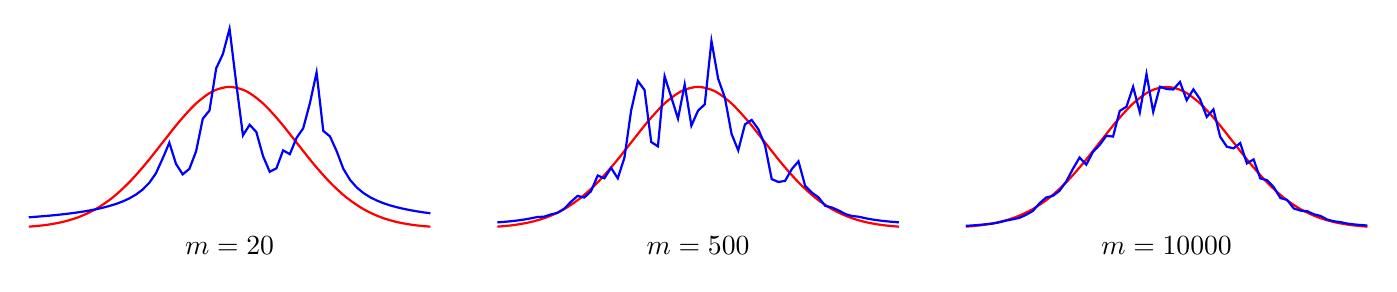
\begin{tikzpicture}[yscale=4.5, xscale=0.85, thick]
		\draw[domain=-3:3, smooth, red, variable=\x] plot ({\x}, {exp(-0.5*\x*\x) * 0.399});
		\draw[blue] (-3.000000, 0.030912) -- (-2.900000, 0.032274) -- (-2.800000, 0.033761) -- (-2.700000, 0.035391) -- (-2.600000, 0.037187) -- (-2.500000, 0.039176) -- (-2.400000, 0.041389) -- (-2.300000, 0.043866) -- (-2.200000, 0.046660) -- (-2.100000, 0.049833) -- (-2.000000, 0.053470) -- (-1.900000, 0.057678) -- (-1.800000, 0.062607) -- (-1.700000, 0.068323) -- (-1.600000, 0.075349) -- (-1.500000, 0.083985) -- (-1.400000, 0.094857) -- (-1.300000, 0.108964) -- (-1.200000, 0.127998) -- (-1.100000, 0.155090) -- (-1.000000, 0.196730) -- (-0.900000, 0.241254) -- (-0.800000, 0.181496) -- (-0.700000, 0.152069) -- (-0.600000, 0.167628) -- (-0.500000, 0.217352) -- (-0.400000, 0.309016) -- (-0.300000, 0.332237) -- (-0.200000, 0.451218) -- (-0.100000, 0.491503) -- (0.000000, 0.562929) -- (0.100000, 0.408311) -- (0.200000, 0.262201) -- (0.300000, 0.292019) -- (0.400000, 0.271548) -- (0.500000, 0.203632) -- (0.600000, 0.159348) -- (0.700000, 0.169086) -- (0.800000, 0.219810) -- (0.900000, 0.209003) -- (1.000000, 0.254695) -- (1.100000, 0.282040) -- (1.200000, 0.352625) -- (1.300000, 0.439682) -- (1.400000, 0.274791) -- (1.500000, 0.259323) -- (1.600000, 0.217551) -- (1.700000, 0.167746) -- (1.800000, 0.136498) -- (1.900000, 0.115063) -- (2.000000, 0.099447) -- (2.100000, 0.087563) -- (2.200000, 0.078216) -- (2.300000, 0.070672) -- (2.400000, 0.064455) -- (2.500000, 0.059244) -- (2.600000, 0.054812) -- (2.700000, 0.050997) -- (2.800000, 0.047679) -- (2.900000, 0.044766) -- (3.000000, 0.042188);
		\node at (0, -0.05) {$m=20$};
		
		\draw[domain=-3:3, smooth, red, variable=\x] plot ({7+\x}, {exp(-0.5*\x*\x) * 0.399});
		\draw[blue] (4.000000, 0.016478) -- (4.100000, 0.017946) -- (4.200000, 0.019702) -- (4.300000, 0.021839) -- (4.400000, 0.024495) -- (4.500000, 0.027887) -- (4.600000, 0.031643) -- (4.700000, 0.032597) -- (4.800000, 0.038892) -- (4.900000, 0.043361) -- (5.000000, 0.055259) -- (5.100000, 0.074456) -- (5.200000, 0.091214) -- (5.300000, 0.086586) -- (5.400000, 0.104425) -- (5.500000, 0.148818) -- (5.600000, 0.141035) -- (5.700000, 0.170552) -- (5.800000, 0.140915) -- (5.900000, 0.199459) -- (6.000000, 0.332479) -- (6.100000, 0.415482) -- (6.200000, 0.390153) -- (6.300000, 0.243308) -- (6.400000, 0.231031) -- (6.500000, 0.428888) -- (6.600000, 0.369657) -- (6.700000, 0.309421) -- (6.800000, 0.405798) -- (6.900000, 0.289492) -- (7.000000, 0.332063) -- (7.100000, 0.349575) -- (7.200000, 0.528778) -- (7.300000, 0.421831) -- (7.400000, 0.368973) -- (7.500000, 0.266194) -- (7.600000, 0.219743) -- (7.700000, 0.292974) -- (7.800000, 0.305682) -- (7.900000, 0.279585) -- (8.000000, 0.234051) -- (8.100000, 0.138772) -- (8.200000, 0.130446) -- (8.300000, 0.133778) -- (8.400000, 0.166943) -- (8.500000, 0.188931) -- (8.600000, 0.119329) -- (8.700000, 0.100467) -- (8.800000, 0.087022) -- (8.900000, 0.063306) -- (9.000000, 0.058376) -- (9.100000, 0.050152) -- (9.200000, 0.040153) -- (9.300000, 0.034502) -- (9.400000, 0.032542) -- (9.500000, 0.028280) -- (9.600000, 0.024798) -- (9.700000, 0.022079) -- (9.800000, 0.019897) -- (9.900000, 0.018108) -- (10.000000, 0.016614);
		\node at (7, -0.05) {$m=500$};
		
		\draw[domain=-3:3, smooth, red, variable=\x] plot ({14+\x}, {exp(-0.5*\x*\x) * 0.399});
		\draw[blue] (11.000000, 0.006779) -- (11.100000, 0.007873) -- (11.200000, 0.009383) -- (11.300000, 0.011256) -- (11.400000, 0.013063) -- (11.500000, 0.016750) -- (11.600000, 0.021479) -- (11.700000, 0.025188) -- (11.800000, 0.029294) -- (11.900000, 0.037798) -- (12.000000, 0.048504) -- (12.100000, 0.070106) -- (12.200000, 0.086664) -- (12.300000, 0.091432) -- (12.400000, 0.105619) -- (12.500000, 0.131789) -- (12.600000, 0.167379) -- (12.700000, 0.199576) -- (12.800000, 0.179463) -- (12.900000, 0.215490) -- (13.000000, 0.235025) -- (13.100000, 0.261005) -- (13.200000, 0.258727) -- (13.300000, 0.331118) -- (13.400000, 0.342982) -- (13.500000, 0.399206) -- (13.600000, 0.327205) -- (13.700000, 0.435013) -- (13.800000, 0.328604) -- (13.900000, 0.399489) -- (14.000000, 0.392978) -- (14.100000, 0.391679) -- (14.200000, 0.412969) -- (14.300000, 0.361395) -- (14.400000, 0.391842) -- (14.500000, 0.364244) -- (14.600000, 0.314217) -- (14.700000, 0.335372) -- (14.800000, 0.258383) -- (14.900000, 0.230056) -- (15.000000, 0.225464) -- (15.100000, 0.240329) -- (15.200000, 0.183084) -- (15.300000, 0.194312) -- (15.400000, 0.140430) -- (15.500000, 0.135825) -- (15.600000, 0.116266) -- (15.700000, 0.085234) -- (15.800000, 0.080030) -- (15.900000, 0.055827) -- (16.000000, 0.049774) -- (16.100000, 0.048143) -- (16.200000, 0.039489) -- (16.300000, 0.034667) -- (16.400000, 0.024548) -- (16.500000, 0.019633) -- (16.600000, 0.017155) -- (16.700000, 0.013106) -- (16.800000, 0.010784) -- (16.900000, 0.009069) -- (17.000000, 0.007646);
		\node at (14, -0.05) {$m=10000$};
	\end{tikzpicture}
\end{center}

\paragraph{k-NN}
On appelle le classificateur des $k$ plus proches voisins k-NN. On note $m_j$ le nombre d'exemples dans la classe $y_j$. De même on note $k_j$ le nombre d'exemples dans la classe $y_j$ qui sont dans l'hypersphère centrée en $x$ qui contient les $k$ plus proches voisins. On a donc :
$$ \sum_j m_j = m \qquad \text{et} \qquad \sum_j k_j = k $$
Ensuite on regarde ce que nous donne la classification bayésienne :
$$ h(x) = \argmax_j \dfrac{\hat{p}(x | y_j) \hat{p}(y_j)}{\hat{p}(x)} = \argmax_j \dfrac{\dfrac{k_j}{m_j \times V} \times \dfrac{m_j}{m}}{\dfrac{k}{m \times V}} = \argmax_j \dfrac{k_j}{k} $$

\begin{center}
	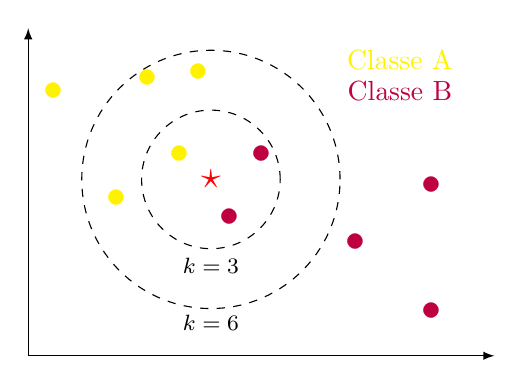
\begin{tikzpicture}[scale=0.8, >={latex}]
		\draw[->] (-0.4, -0.2) -- (7, -0.2);
		\draw[->] (-0.4, -0.2) -- (-0.4, 5);
		\node[yellow] at (0, 4) {\Large $\bullet$};
		\node[yellow] at (1, 2.3) {\Large $\bullet$};
		\node[yellow] at (1.5, 4.2) {\Large $\bullet$};
		\node[yellow] at (2, 3) {\Large $\bullet$};
		\node[yellow] at (2.3, 4.3) {\Large $\bullet$};
		\node[red] at (2.5, 2.6) {\Large $\star$};
		\node[purple] at (2.8, 2) {\Large $\bullet$};
		\node[purple] at (3.3, 3) {\Large $\bullet$};
		\node[purple] at (4.8, 1.6) {\Large $\bullet$};
		\node[purple] at (6, 2.5) {\Large $\bullet$};
		\node[purple] at (6, 0.5) {\Large $\bullet$};
		
		\draw[dashed] (2.5, 2.6) circle (1.1);
		\draw[dashed] (2.5, 2.6) circle (2.05);
		\node[below] at (2.5, 1.5) {\footnotesize $k=3$};
		\node[below] at (2.5, 0.6) {\footnotesize $k=6$};
		\node[yellow!100] at (5.5, 4.5) {Classe A};
		\node[purple!100] at (5.5, 4) {Classe B};
	\end{tikzpicture}
\end{center}

\PROP{
	L'erreur de généralisation $\epsilon_{1NN}$ du 1-plus proche voisin est bornée par deux fois l'erreur de Bayes $\epsilon_B$ lorsque $m$ tend vers l'infini :
	$$2 \epsilon_B - 2 \epsilon_B^2 \leqslant \epsilon_{1NN} \leqslant 2 \epsilon_B - \epsilon_B^2$$
	\vspace{-5mm}
}

\dem
Soit $x \in \X$ et $y$ sa classe c'est à dire $y = \argmax_{y_j} p(y_j | x)$. L'erreur de Bayes est la suivante :
$$ \epsilon_B(x) = \sum_{y_j \neq y} p(y_j | x) $$
L'erreur de l'algorithme 1-plus proche voisin est la suivante :
$$ \epsilon_{1NN} = 1 - \sum_j p(y_j | x) p(y_j | x') $$
où $x'$ est le plus proche voisin de $x$. Quand $m$ tend vers l'infini, $x'$ tend vers $x$. Cela nous donne :
$$ \epsilon_{1NN} \simeq 1 - \sum_j p(y_j | x)^2 = 1 - p(y|x)^2 - \sum_{y_j \neq y} p(y_j | x)^2 $$
Or $p(y | x) = 1 - \epsilon_B$ et on peut borner la somme qui intervient dans $\epsilon_{1NN}$. En effet soit un ensemble $\{ v_i \}$ de valeurs positives tel que $\sum_i v_i = a$. On a :
$$ \left( \sum_i v_i \right)^2 = a^2 $$
On développe la somme au carré et on obtient :
$$ 0 \leqslant \sum_i v_i^2 = a^2 - 2 \sum_{i \neq j} v_i v_j \leqslant a^2 $$.
Dans notre cas, cela donne :
$$ 0 \leqslant \sum_{y_j \neq y} p(y_j | x)^2 \leqslant \epsilon_B^2 $$
Finalement en reprenant notre expression de $\epsilon_{1NN}$ on obtient :
$$ 1 - (1 - \epsilon_B)^2 - \epsilon_B^2 \leqslant \epsilon_{1NN} \leqslant 1 - (1 - \epsilon_B)^2 $$
Ce qui nous donne les inégalités souhaitées.
\findem

\paragraph{Effet de $k$} De plus l'erreur asymptotique diminue lorsque $k$ augmente.
$$ \epsilon_B \leqslant \epsilon_{kNN} \leqslant \epsilon_{(k-1)NN} \leqslant ... \leqslant \epsilon_{1NN} \leqslant 2 \epsilon_B $$
Le graphique ci dessous nous montre l'erreur pour différentes valeurs de $k$ pour classification binaire ($|\Y| = 2$).
\begin{center}
	\begin{tikzpicture}[yscale=7, xscale=9, thick, >={latex}]
		\draw[->] (0, 0) -- (0.55, 0);
		\draw[->] (0, 0) -- (0, 0.55);
		\draw[red, ultra thick] (0, 0) -- (0.5, 0.5);
		\draw[red] (0.32, 0.1) node {\footnotesize Erreur de Bayes};
		\draw[->, red] (0.32, 0.14) -- (0.27, 0.26);
		\draw[] (0.25, 0.02) -- (0.25, -0.02) node[below] { \footnotesize 0.25};
		\draw[] (0.5, 0.025) -- (0.5, -0.025) node[below] { \footnotesize 0.5};
		\draw[] (0.019, 0.5) -- (-0.019, 0.5) node[left] { \footnotesize 0.5};
		\draw[] (0.015, 0.25) -- (-0.015, 0.25) node[left] { \footnotesize 0.25};
		\draw[blue] (0.000000, 0.000000) -- (0.016667, 0.032778) -- (0.033333, 0.064444) -- (0.050000, 0.095000) -- (0.066667, 0.124444) -- (0.083333, 0.152778) -- (0.100000, 0.180000) -- (0.116667, 0.206111) -- (0.133333, 0.231111) -- (0.150000, 0.255000) -- (0.166667, 0.277778) -- (0.183333, 0.299444) -- (0.200000, 0.320000) -- (0.216667, 0.339444) -- (0.233333, 0.357778) -- (0.250000, 0.375000) -- (0.266667, 0.391111) -- (0.283333, 0.406111) -- (0.300000, 0.420000) -- (0.316667, 0.432778) -- (0.333333, 0.444444) -- (0.350000, 0.455000) -- (0.366667, 0.464444) -- (0.383333, 0.472778) -- (0.400000, 0.480000) -- (0.416667, 0.486111) -- (0.433333, 0.491111) -- (0.450000, 0.495000) -- (0.466667, 0.497778) -- (0.483333, 0.499444) -- (0.500000, 0.500000);
		\draw[blue] (0.52, 0.4) -- (0.56, 0.4) node[right] {\small $k=1$};
		\draw[purple] (0.000000, 0.000000) -- (0.016667, 0.017463) -- (0.033333, 0.036375) -- (0.050000, 0.056525) -- (0.066667, 0.077709) -- (0.083333, 0.099730) -- (0.100000, 0.122400) -- (0.116667, 0.145537) -- (0.133333, 0.168968) -- (0.150000, 0.192525) -- (0.166667, 0.216049) -- (0.183333, 0.239389) -- (0.200000, 0.262400) -- (0.216667, 0.284945) -- (0.233333, 0.306894) -- (0.250000, 0.328125) -- (0.266667, 0.348523) -- (0.283333, 0.367982) -- (0.300000, 0.386400) -- (0.316667, 0.403685) -- (0.333333, 0.419753) -- (0.350000, 0.434525) -- (0.366667, 0.447931) -- (0.383333, 0.459908) -- (0.400000, 0.470400) -- (0.416667, 0.479360) -- (0.433333, 0.486746) -- (0.450000, 0.492525) -- (0.466667, 0.496672) -- (0.483333, 0.499167) -- (0.500000, 0.500000);
		\draw[purple] (0.52, 0.35) -- (0.56, 0.35) node[right] {\small $k=3$};
		\draw[] (0.000000, 0.000000) -- (0.016667, 0.016667) -- (0.033333, 0.033338) -- (0.050000, 0.050030) -- (0.066667, 0.066781) -- (0.083333, 0.083650) -- (0.100000, 0.100713) -- (0.116667, 0.118056) -- (0.133333, 0.135771) -- (0.150000, 0.153940) -- (0.166667, 0.172633) -- (0.183333, 0.191897) -- (0.200000, 0.211749) -- (0.216667, 0.232171) -- (0.233333, 0.253107) -- (0.250000, 0.274464) -- (0.266667, 0.296105) -- (0.283333, 0.317860) -- (0.300000, 0.339523) -- (0.316667, 0.360861) -- (0.333333, 0.381615) -- (0.350000, 0.401516) -- (0.366667, 0.420283) -- (0.383333, 0.437639) -- (0.400000, 0.453314) -- (0.416667, 0.467055) -- (0.433333, 0.478635) -- (0.450000, 0.487858) -- (0.466667, 0.494564) -- (0.483333, 0.498635) -- (0.500000, 0.500000);
		\draw[] (0.52, 0.3) -- (0.56, 0.3) node[right] {\small $k=9$};
		\draw[greenTikz] (0.000000, 0.000000) -- (0.016667, 0.016667) -- (0.033333, 0.033333) -- (0.050000, 0.050000) -- (0.066667, 0.066667) -- (0.083333, 0.083333) -- (0.100000, 0.100000) -- (0.116667, 0.116667) -- (0.133333, 0.133335) -- (0.150000, 0.150006) -- (0.166667, 0.166686) -- (0.183333, 0.183388) -- (0.200000, 0.200137) -- (0.216667, 0.216977) -- (0.233333, 0.233975) -- (0.250000, 0.251225) -- (0.266667, 0.268844) -- (0.283333, 0.286963) -- (0.300000, 0.305703) -- (0.316667, 0.325148) -- (0.333333, 0.345309) -- (0.350000, 0.366087) -- (0.366667, 0.387241) -- (0.383333, 0.408374) -- (0.400000, 0.428930) -- (0.416667, 0.448226) -- (0.433333, 0.465495) -- (0.450000, 0.479952) -- (0.466667, 0.490877) -- (0.483333, 0.497686) -- (0.500000, 0.500000);
		\draw[greenTikz] (0.52, 0.25) -- (0.56, 0.25) node[right] {\small $k=27$};
		\node[below left] at (0, 0) {0};
	\end{tikzpicture}
\end{center}
Comme la propriété précédente n'est valide que lorsque $m$ est suffisamment grand. Il nous faut alors un compromis pour que l'inégalité tienne sans que $m$ soit trop grand. On prend généralement $k = \sqrt{\dfrac{m}{|\Y|}}$.

\paragraph{Problèmes}
Pour faire face à la malédiction de la dimensionnalité, il faut réduire la dimension avec des algorithmes comme PCA. Pour converger l'algorithme des k-plus proches voisins a besoin de beaucoup d'exemples. Cependant, un large nombre d'exemples d'entraînement implique une complexité spatiale et temporelle élevée. Pour résoudre ça, on peut utiliser les deux stratégies suivantes :
\begin{itemize}
	\item Réduire la taille $S$ en ne gardant que les exemples les plus révélateurs.
	\item Simplifier le calcul des plus proches voisins.
\end{itemize}

\paragraph{Étape préliminaire}
La première étape consiste en la suppression des exemples qui sont aberrants ou qui sont dans la région de l'erreur de Bayes.
\begin{center}
	\begin{algorithm}[H]
		\KwIn{$S$}
		\KwOut{$S_{cleaned}$}
		Séparer aléatoirement $S$ en deux parties $S_1$ et $S_2$\;
		\Repeat{stabilisation de $S_1$ et $S_2$}{
			Classer $S_1$ en utilisant 1-NN avec $S_2$\;
			Supprimer de $S_1$ les instances mal classées\;
			Classer $S_2$ en utilisant 1-NN avec le nouvel ensemble $S_1$\;
			Supprimer de $S_2$ les instances mal classées\;
		}
		\KwResult{$S_{cleaned} = S_1 \cup S_2$}
		\caption{Réduction de données}
	\end{algorithm}
	
	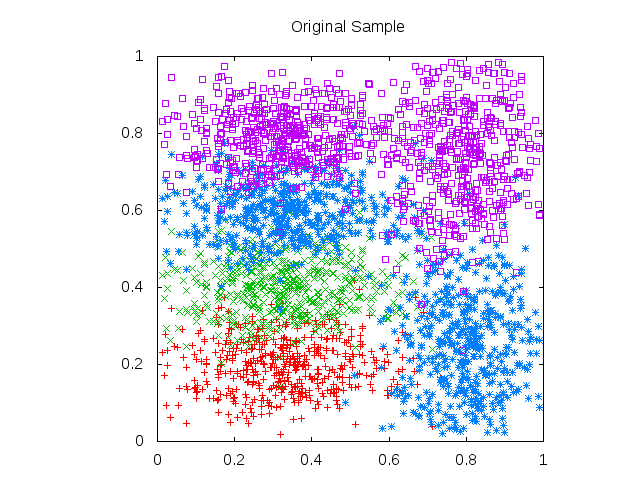
\includegraphics[scale=0.35]{big_samples.png}
	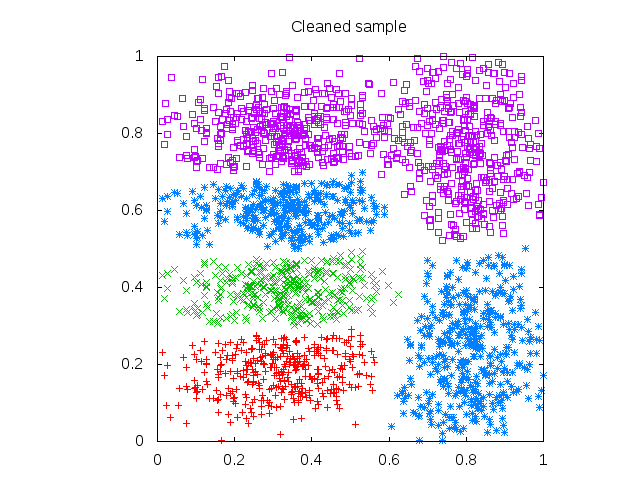
\includegraphics[scale=0.35]{cleaned_samples.png}
\end{center}

\paragraph{Seconde étape}
Puis on supprimer les exemples qui ne sont pas très révélateurs.
\begin{center}
	\begin{algorithm}[H]
		\KwIn{$S$}
		\KwOut{STORAGE}
		STORAGE $\gets \emptyset$\; 
		Choisir aléatoirement un exemple de $S$ et le mettre dans STORAGE\;
		\Repeat{stabilisation de STORAGE}{
			\For{$x \in S$} {
				\If{$x$ n'est pas correctement classé en utilisant 1-NN avec STORAGE}{
					STORAGE $\gets$ STORAGE $\cup \; \{x\}$
				}
			}
		}
		\KwResult{STORAGE}
		\caption{Plus proche voisin condensé (CNN)}
	\end{algorithm}
	
	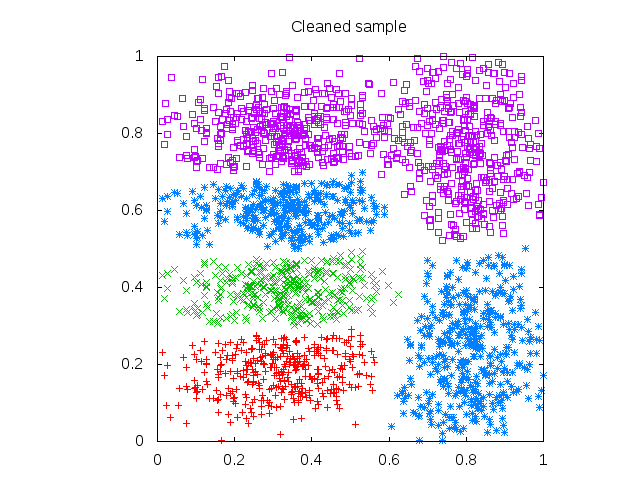
\includegraphics[scale=0.35]{cleaned_samples.png}
	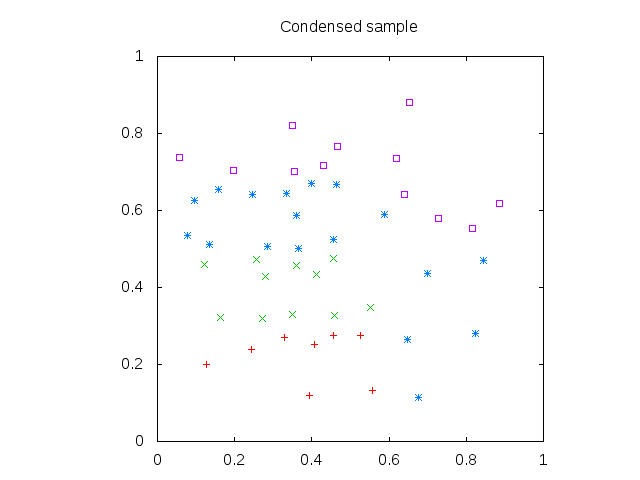
\includegraphics[scale=0.35]{condensed_samples.png}
\end{center}

\paragraph{Augmenter la rapidité}
En 2D ou en 3D on peut utiliser des diagrammes de Voronoi ou encore des graphes de proximité.
En plus grande dimension on peut utiliser les structures de données suivantes : ball-trees, kd-trees, metric-trees, quadtrees et R-trees.

\paragraph{Classification naïve bayésienne}
La classification naïve bayésienne suppose en plus que les features sont indépendantes.
$$ \hat{y}(x_1, ..., x_n) = \argmax_c \prod_{i=1}^n p(x_i | y_c).p(y_c) $$
Cette classification est beaucoup moins sensible à la dimension comme chaque probabilité peut être estimée comme une distribution de dimension 1. Il n'y a alors plus de malédiction de la dimensionnalité. De plus cela rend plus lisse la probabilité obtenue.

\paragraph{Question} Comment peut-on améliorer la qualité de la métrique utilisée dans k-NN ?

\sect{Apprentissage de métriques}

On commence par rappeler ce q'est une distance sur un espace $X$.

\DEF{
	Une \textbf{métrique/distance} sur un espace $X$ est une fonction positive $d : X \times X \rightarrow \R_+$ qui vérifie les conditions suivantes :
	\begin{itemize}
		\item Positivité : $d(x, y) \geqslant 0$
		\item Séparation : $d(x, y) = 0 \Leftrightarrow x = y$
		\item Symétrie : $d(x, y) = d(y, x)$
		\item Inégalité triangulaire : $d(x, z) \leqslant d(x, y) + d(y, z)$
	\end{itemize}
}

Les normes $l_p$ sont des distances. La norme $l_1$ est appelée \textbf{distance de Manhattan}, la norme $l_2$ est appelée \textbf{distance euclidienne} et la norme $l_\infty$ est appelée \textbf{distance de Tchebychev}. \\
Mais comment choisir la bonne métrique ? L'idée est d'apprendre une métrique qui assigne une faible distance aux paires d'exemples qui sont sémantiquement similaire (par exemple qui ont la même classe dans le cas de la classification supervisée) et qui assigne une distance élevée aux paires d'exemples qui ne sont sémantiquement différents.

\begin{center}
	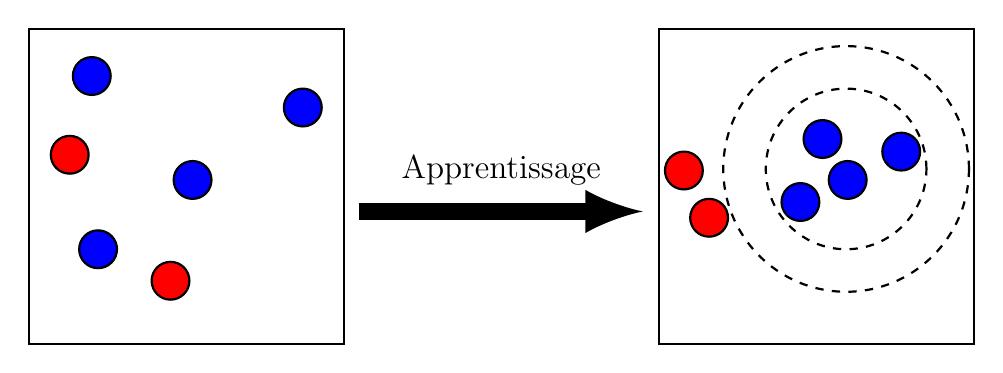
\begin{tikzpicture}[scale=4, thick, >={latex}]
		\draw[fill=red] (0.45, 0.2) circle (0.06);
		\draw[fill=red] (0.13, 0.6) circle (0.06);
		\draw[fill=blue] (0.22, 0.3) circle (0.06);
		\draw[fill=blue] (0.52, 0.52) circle (0.06);
		\draw[fill=blue] (0.2, 0.85) circle (0.06);
		\draw[fill=blue] (0.87, 0.75) circle (0.06);
		\draw (0, 0) rectangle (1, 1);
		\draw[fill=red] (2.08, 0.55) circle (0.06);
		\draw[fill=red] (2.16, 0.4) circle (0.06);
		\draw[fill=blue] (2.45, 0.45) circle (0.06);
		\draw[fill=blue] (2.6, 0.52) circle (0.06);
		\draw[fill=blue] (2.52, 0.65) circle (0.06);
		\draw[fill=blue] (2.77, 0.61) circle (0.06);
		\draw[dashed] (2.595, 0.555) circle (0.255);
		\draw[dashed] (2.595, 0.555) circle (0.39);
		\draw (2, 0) rectangle (3, 1);
		
		\node at (1.5, 0.55) {\large Apprentissage};
		\draw[line width=6, ->] (1.05, 0.42) -- (1.95, 0.42);
	\end{tikzpicture}
\end{center}

\DEF{
	La \textbf{distance de Mahalanobis} est définie de la manière suivante :
	$$ d_M(x, x') = \sqrt{(x - x')^\trans M (x - x')} $$
	Où $M \in \R^{d \times d}$ est une matrice symétrique définie positive.
}

Cette distance vient du cas où $x$ et $x'$ suivent la même distribution de matrice de covariance $\Sigma$ et dans ce cas $M = \Sigma^{-1}$. \\
On peut décider de prendre $M$ uniquement positive et pas définie positive, c'est à dire autoriser $M$ à avoir des valeurs propres nulles. Cela permet de faire une réduction de dimension. \\
De plus comme $M$ est symétrique positive on peut l'écrire de la manière suivante : $M = L^\trans L$. Dans ce cas en posant $\tilde{x} = Lx$, on a :
$$ \begin{array}{lll}
d_M(x, x')
& = & \sqrt{(x - x')^\trans L^\trans L (x - x')} \\
& = & \sqrt{(Lx - Lx')^\trans (Lx - Lx')} \\
& = & \sqrt{(\tilde{x} - \tilde{x}')^\trans (\tilde{x} - \tilde{x}')} \\
& = & d_{euc}(\tilde{x}, \tilde{x}')
\end{array} $$

\paragraph{Apprentissage}
Désormais, étant donnée une métrique paramétrisée par $M$, on va essayer de résoudre le problème d'optimisation suivant:
$$ M^*=\argmin_{M \succeq 0} l(M, \mathcal{S}, \mathcal{D}, \mathcal{R}) + \lambda R(M) $$
Où $l$ est une fonction de perte qui pénalise des contraintes violées, $R$ est un régularisateur de $M$ et $\lambda$ est un paramètre qui permet de contrôler l'importance de la régularisation. L'état de l'art se différencie alors par les choix de la fonction de perte, des contraintes et du régularisateur. \\
Les contraintes sont les suivantes :
\begin{itemize}
	\item $\displaystyle \mathcal{S} = \left\{ (x, x')~|~x \text{ et } x' \text{ sont similaires} \right\}$
	\item $\displaystyle \mathcal{D} = \left\{ (x, x')~|~x \text{ et } x' \text{ sont éloignés} \right\}$
	\item $\displaystyle \mathcal{R} = \left\{ (x, x', x'')~|~x \text{ est plus proche de } x' \text{ que de } x'' \right\}$
\end{itemize}
Les régularisateurs usuels sont les suivants :
\begin{itemize}
	\item La norme de Frobenius (simple et classique) $\| M \|_\mathcal{F}^2 = \sum_{i, j} M_{ij}^2$.
	\item La sélections de features avec la norme mixe $L_{2, 1}$ : $\| M \|_{2, 1} = \sum_i \| M_i \|_2$. \\ Cette norme est bien convexe mais elle n'est pas lisse.
	\item La favorisation des matrices de rang faible pour la réduction de dimension \\
		$\| M \|_* = tr(M) = \sum_i \sigma_i(M) $.
	\item L'utilisation de la LogDet divergence.
\end{itemize}

\paragraph{LMNN}
L'algorithme LMNN considère les ensembles de contraintes suivants :
$$ \mathcal{S} = \left\{ (x_i, x_j)~|~y_i = y_j \text{ et } x_j \text{ appartient aux } k \text{ plus proches voisins de } x_i \right\} $$
$$ \mathcal{R} = \left\{ (x_i, x_j, x_k)~|~(x_i, x_j) \in \mathcal{S}, \, y_i \neq y_k \right\} $$
La formulation stricte est alors la suivante :
$$ \min_{M \succeq 0} \quad \sum_{(x_i, x_j) \in \mathcal{S}} d_M^2(x_i, x_j) $$
\vspace{-4mm}
$$ s.t. \quad \forall (x_i, x_j, x_k) \in \mathcal{R}, \; d_M^2(x_i, x_k) - d_M^2(x_i, x_j) \geqslant 1 $$
La formulation douce est la suivante :
$$ \min_{M \succeq 0} \quad (1 - \mu) \sum_{(x_i, x_j) \in \mathcal{S}} d_M^2(x_i, x_j) + \mu \sum_{i, j, k} \xi_{ijk} $$
\vspace{-4mm}
$$ s.t. \quad \forall (x_i, x_j, x_k) \in \mathcal{R}, \; d_M^2(x_i, x_k) - d_M^2(x_i, x_j) \geqslant 1 - \xi_{ijk} $$
Où $\mu$ contrôle la contrepartie entre attirer les exemples proches et éloigner les exemples d'étiquettes différentes. \\
L'avantage de cet apprentissage est qu'il est convexe et qu'il possède un solveur efficace même pour un large nombre de contraintes. Le désavantage est qu'il est soumis à l'overfitting lorsque la dimension est élevée.

\paragraph{ITML} L'Information-Thoretical Metric Learning introduit une régularisation utilisant la divergence LogDet définie par :
$$ D_{id}(M, M_0) = tr \left (MM_0^{-1} \right) - \log \det \left( MM_0^{-1} \right) - d $$
Où $d$ est la dimension et $M_0$ est une matrice symétrique positive dont on veut rester proche. L'ITML est formulé de la manière suivante :
$$ \min_{M \succeq 0} \quad D_{id}(M, M_0) $$
\vspace{-4mm}
$$ s.t. \quad \left\{ \begin{array}{ll}
	\forall (x_i, x_j) \in \mathcal{S} & d_M^2(x_i, x_j) \leqslant u \\
	\forall (x_i, x_j) \in \mathcal{D} & d_M^2(x_i, x_j) \geqslant v
\end{array} \right.$$

\paragraph{Non-linéarité}
LMNN et ITML génèrent des transformations linéaires qui sont incapable ce capturer des structures non linéaires dans les données. Comme solution à ce problème on peut utiliser des noyaux comme KPCA (PCA dans un espace noyau) ou des métriques locales. Pour les métriques locales on peut par exemples partitionner notre ensemble en C clusters puis apprendre une distance de Mahalanobis sur chacun de ces clusters.